% Jinja Template for Latex file
% Copyright François Pacaud, 2023

\documentclass{article}

\usepackage{amsmath,amsfonts,amssymb,amsthm}
\usepackage{xcolor,bm,url}
\usepackage{booktabs}
\usepackage{tikz}

\newtheorem{theorem}{Theorem}[section]
\newtheorem{lemma}[theorem]{Lemma}
\newtheorem{corollary}[theorem]{Corollary}
\newtheorem{proposition}[theorem]{Proposition}
\theoremstyle{definition}
\newtheorem{definition}[theorem]{Definition}
\newtheorem{example}[theorem]{Example}
\theoremstyle{remark}
\newtheorem{remark}{Remark}

\DeclareMathOperator{\diag}{diag}
\DeclareMathOperator{\argmin}{arg\,min}

\title{Nonlinear programming on GPU: current state-of-the-art}
\author{TBD}
\date{\today}

\begin{document}
\maketitle

\begin{abstract}
  Solving generic nonlinear programs requires the
  successive solution of large-scale indefinite symmetric matrix.
  The sparse factorization of such matrices relies
  on expensive numerical pivoting operations
  which are notoriously hard to parallelize on a GPU.
  A workaround is to reformulate the successive KKT systems
  in a form more amenable for the GPU, either by densifying
  it using a null-space method or by reducing it down
  to a symmetric positive-definite system, whose factorization using
  Cholesky run efficiently on the GPU.
  In this paper, we test three concurrent methods for solving
  KKT systems on the GPU using the newly released cuDSS solver,
  which implements the three sparse factorization routines LU, LDL
  and Cholesky, all offering uncompromising performance on NVIDIA GPU.
  We benchmark the three methods using various large-scale nonlinear programs,
  taken from the PGLIB and COPS benchmarks.
  We illustrate the advantages and the downsides of the three methods.
  We find that GPUs shine to compute quick and dirty results down to a medium convergence tolerance
  --- with a 10x speed-up compared to a state-of-the-art CPU routine --- but
  with a limited robustness.
\end{abstract}


% \tableofcontents


\section{Introduction}
Graphics processing units (GPUs) are driving the advancement of scientific computing, their most remarkable success being the capabilities to train and utilize large artificial intelligence (AI) models.
GPUs offer several practical advantages: (1) massive parallel computing capability for applications that can exploit coarse-grain parallelism and high-memory bandwidth and (2) power efficiency due to requiring fewer transistors to process multiple tasks in parallel utilizing ``single instruction, multiple data'' (SIMD) parallelism.

While GPUs have made significant strides in enhancing machine learning applications, their adoption in the mathematical programming community has been relatively limited.
This limitation stems primarily from the fact that most optimization solvers were developed in the 1990s and are heavily optimized for CPU architectures.
Additionally, the utilization of GPUs has been impeded by the challenges associated with sparse matrix factorization routines, which are inherently difficult to parallelize on SIMD architectures. Nevertheless, recent years have witnessed notable advancements that are reshaping this landscape.
\begin{enumerate}
  \item \textbf{Improved sparse matrix operations}: The performance of sparse matrix operations has seen substantial improvements in the CUDA library, largely attributed to the integration of novel tensor cores in recent GPUs~\cite{markidis2018nvidia}.
  \item \textbf{Interest in batch optimization}: There is a growing interest in solving parametric optimization problems in batch mode, for problems sharing the same structure but with different parameters~\cite{amos2017optnet,pineda2022theseus}.
  \item \textbf{Advancements in automatic differentiation}: GPUs offer unparalleled performance for automatic differentiation, benefiting both machine learning~\cite{jax2018github} and scientific computing applications \cite{enzyme2021}. Engineering problems often exhibit recurring patterns throughout the model. Once these patterns are identified, they can be evaluated in parallel within a SIMD framework, enabling near speed-of-light performance~\cite{shin2023accelerating}.
  \item \textbf{Role in exascale computing}: With the emergence of new exascale supercomputers (e.g., Frontier and Aurora), the capabilities to run on GPUs have become even more important for supercomputing.
\end{enumerate}

\subsection{Solving optimization problems on GPU: current state-of-the-art}
For all the reasons listed before, there is an increasing interest to solve optimization problems on GPUs.
We now summarize the previous work on solving classical---large-scale, sparse, constrained---mathematical programs on GPUs.

\paragraph{GPU for mathematical programming.}
The factorization of sparse matrices encountered within second-order optimization algorithms has been considered to be challenging  on GPUs.
For this reason, practitioners often has resorted to using first-order
methods on GPUs, leveraging level-1 and level-2 BLAS operations that
are more amenable to parallel computation.
First-order algorithms depend mostly on (sparse) matrix-vector operations that run
very efficiently on modern GPUs. Hence, we can counterbalance
the relative inaccuracy of the first-order method by running more
iterations of the algorithm.
A recent breakthrough~\cite{lu2023cupdlp,lu2023cupdlp2} based on the primal-dual hybrid gradient method has demonstrated
that a first-order algorithm can surpass the performance of Gurobi, a
commercial solver, in tackling large-scale linear programs. This
performance gain is made possible by executing the first-order
iterations solely on the GPU through an optimized codebase.

\paragraph{GPU for batched optimization solvers.}
The machine learning community has been a strong advocate for porting
mathematical optimization on the GPU. One of the most promising
applications is embedding mathematical programs inside neural networks,
a task that requires batching the solution of the optimization model
for the training algorithm to be
efficient~\cite{amos2017optnet,pineda2022theseus}.  This has led to
the development of prototype code solving thousands of (small)
optimization problems in parallel on the GPU.
Furthermore, batched optimization solvers can be leveraged
in decomposition algorithms, when the subproblems share the same structure~\cite{kimLeveragingGPUBatching2021}.
However, it is not trivial to adapt such code to solve large-scale optimization problems,
as the previous prototypes are reliant on dense linear solvers to
compute the descent directions.

\paragraph{GPU for nonlinear programming.}
The success of first-order algorithms in classical mathematical programming
relies on the convexity of the problem. Thus, this approach is nontrivial to replicate
in nonlinear programming: Most engineering problems encode complex
physical equations that are likely to break any convex structure in the problem.
Previous experiments on the alternating current (AC) optimal power flow (OPF) problem have shown that even a simple
algorithm as an alternating direction method of multipliers (ADMM) has trouble converging as soon as the convergence
tolerance is set below $10^{-3}$~\cite{kimLeveragingGPUBatching2021}.

Thus, second-order methods remain a competitive option, particularly
for scenarios that require higher levels of accuracy and robust convergence.
Second-order algorithms require solving a Newton step at each
iteration, an operation relying on non-trivial sparse linear algebra operations.
The previous generation of GPU-accelerated sparse linear
solvers were lagging behind their CPU equivalents, as illustrated in
subsequent surveys~\cite{swirydowicz2021linear,tasseff2019exploring}.
Fortunately, sparse solvers on GPUs are becoming increasingly better: NVIDIA has released in November 2023
the {\tt cuDSS} sparse direct solver that implements different sparse factorization routines with remarkably improved performance.
Our benchmark results incidate that {\tt cuDSS} is significantly faster than the previous sparse solvers using NVIDIA GPUs (e.g., published in \cite{shin2023accelerating}).
% SS: removed due to irrelevance.
% The new NVIDIA Grace CPU architecture could also be a game changer in the future of sparse linear solvers, thanks to fast communication between the CPU and GPU.
Furthermore, variants of interior point methods have been proposed
that does not require the use of numerical pivoting in the linear solves,
opening the door to parallelized sparse solvers.
Coupled with a GPU-accelerated automatic differentiation library and a
sparse Cholesky solver, these nonlinear programming solvers can solve
optimal power flow (OPF) problems 10x faster than state-of-the-art
methods~\cite{shin2023accelerating}.

There exist a few alternatives to sparse linear solvers for solving the KKT systems on the GPU.
On the one hand, iterative and Krylov methods rely only on matrix-vector products to solve linear systems.
They often require non-trivial reformulation or
specialized preconditioning of the KKT systems to mitigate the
inherent ill-conditioning of the KKT matrices, which has limited their
use within the interior-point methods
\cite{curtisNoteImplementationInteriorpoint2012,rodriguezScalablePreconditioningBlockstructured2020}.
New results are giving promising outlooks for convex problems~\cite{ghannad2022linear},
but nonconvex problems often require an Augmented Lagrangian reformulation
to be tractable~\cite{cao2016augmented,regev2023hykkt}. In particular,
\cite{regev2023hykkt} presents an interesting use of the Golub and Greif
hybrid method~\cite{golub2003solving} to solve the KKT systems arising in
the interior-point methods, with promising results on the GPU.
On the other hand, null-space methods (also known as reduced Hessian methods)
reduce the KKT system down to a dense matrix, a setting also favorable for GPUs.
Our previous research has shown that the method plays nicely with the interior-point
methods if the number of degrees of freedom in the problem is relatively small~\cite{pacaud2022condensed}.


\subsection{Contributions}
In this article, we assess the current capabilities of modern GPUs
to solve large-scale nonconvex nonlinear programs to optimality.
We focus on the two condensed-space methods
introduced respectively in~\cite{regev2023hykkt,shin2023accelerating}.
We re-use classical results from~\cite{wright1998ill} to show
that for both methods, the condensed matrix exhibits
structured ill-conditioning that limits the loss of accuracy in
the descent direction (provided the interior-point algorithm satisfies
some standard assumptions).
We implement both algorithms inside the GPU-accelerated solver MadNLP,
and leverage the GPU-accelerated automatic differentiation
backend ExaModels~\cite{shin2023accelerating}.
The interior-point algorithm runs entirely on the GPU, from
the evaluation of the model (using ExaModels) to the solution of
the KKT system (using a condensed-space method running on the GPU).
We use CUDSS.jl \cite{Montoison_CUDSS}, a Julia interface to the NVIDIA library {\tt cuDSS},
to solve the condensed KKT systems. We evaluate the strengths
and weaknesses of both methods, in terms of accuracy and runtime.
Extending beyond the classical OPF instances examined in our previous work,
we incorporate large-scale problems sourced from the COPS nonlinear benchmark~\cite{dolan2004benchmarking}.
Our assessment involves comparing the performance achieved on the GPU with that of a state-of-the-art method executed on the CPU.
The findings reveal that the condensed-space IPM enables a remarkable 10x acceleration in solving large-scale OPF instances when utilizing the GPU.
However, performance outcomes on the COPS benchmark exhibit more variability.

\subsection{Notations}
By default, the norm $\|\cdot\|$ refers to the 2-norm.
We define the conditioning of a matrix $A$ as
$\cond(A) = \| A \| \|A^{-1} \|$. % Sungho: I wonder if subscript 2 is necessary in that it is clear from the context that we're connsidering 2 norm.
For any real number $x$, we denote by $\widehat{x}$ its floating
point representation.
We denote $\epstol$ as the smallest positive number such that
$\widehat{x} \leq (1 + \tau) x$ for $|\tau| < \epstol$.
In double precision, $\epstol = 1.1 \times 10^{-16}$.
We use the following notations to proceed with our error analysis.
For $p \in \mathbb{N}$ and a positive variable $h$:
\begin{itemize}
  \item We write $x = O(h^p)$ if there exists a constant $b > 0$
    such that $\| x \| \leq b h^p$;
  \item We write $x = \Omega(h^p)$ if there exists a constant $a > 0$
    such that $\| x \| \geq a h^p$;
  \item We write $x = \Theta(h^p)$ if there exists two constants $0 < a < b$
    such that $a h^p \leq \| x \| \leq b h^p$.
\end{itemize}

%%% Local Variables:
%%% mode: LaTeX
%%% TeX-master: "../main.tex"
%%% End:

\section{Primal-dual interior-point method}
The interior-point method (IPM) is among the most popular algorithm
to solve nonlinear program. The basis of the algorithm is to
reformulate the KKT conditions of the nonlinear program as a smooth
system of nonlinear equations~\cite{nocedal_numerical_2006}. In a standard implementation, the
resulting system is solved iteratively with a Newton method used in conjunction
with a line-search method for globalization. In this section, we
give a brief description of a nonlinear program in \S\ref{sec:ipm:problem}
and detail the Newton step solved at each IPM iteration in \S\ref{sec:ipm:kkt}.

\subsection{Problem's formulation and KKT conditions ( FP)}
\label{sec:ipm:problem}
We are interested in solving the following nonlinear program:
\begin{equation}
  \label{eq:problem}
    \min_{x \in \mathbb{R}^n} \;  f(x)
\quad \text{subject to}\quad
\left\{
  \begin{aligned}
    & g(x) = 0 \; , ~ h(x) \leq 0 \\
      & x \geq 0  \; ,
  \end{aligned}
\right.
\end{equation}
with $f:\mathbb{R}^n \to \mathbb{R}$ a real-valued function
encoding the objective, $g: \mathbb{R}^n \to \mathbb{R}^{m_e}$
a function defining the equality constraints, and $h: \mathbb{R}^{n} \to
\mathbb{R}^{m_i}$ a function encoding the inequality constraints.
In addition, the variable $x$ is subject to simple bounds $x \geq 0$.
In what follows, we suppose that the functions $f, g, h$ are smooth
and twice differentiable.

By introducing a set of slack variables $s \geq 0$, the problem
\eqref{eq:problem} is equivalent to
\begin{equation}
  \label{eq:slack_problem}
    \min_{x \in \mathbb{R}^n, s \in \mathbb{R}^{m_i}} \;  f(x)
    \quad \text{subject to} \quad
    \left\{
  \begin{aligned}
    & g(x) = 0 \; , ~ h(x) + s = 0 \\
      & x \geq 0  \; , ~ s \geq 0  \; .
  \end{aligned}
  \right.
\end{equation}
Using the formulation~\eqref{eq:slack_problem}, the inequality constraints
are directly encoded inside the variable bounds.

In \eqref{eq:slack_problem},
we note by $y \in \mathbb{R}^{m_e}$ the multipliers associated
to the equality constraints and $z \in \mathbb{R}^{m_i}$ the multipliers
associated to the inequality constraints. Similarly, we note
by $(u, v) \in \mathbb{R}^{n + m_i}$ the multipliers associated
respectively to the bounds on the variables $x$ and the slacks $s$.
Using the dual multipliers $(y, z, v, w)$,
the Lagrangian of \eqref{eq:slack_problem} writes out
\begin{equation}
  \label{eq:lagrangian}
  L(x, s; y, z, u, v) = f(x) + y^\top g(x) + z^\top \big(h(x) +s\big)
  - u^\top x - v^\top s \; .
\end{equation}
The KKT conditions of \eqref{eq:slack_problem} are:
\begin{subequations}
  \label{eq:kktconditions}
    \begin{align}
      & \nabla f(x) + \nabla g(x)^\top y + \nabla h(x)^\top z - v = 0 \\
      & z - w = 0 \\
      & g(x) = 0 \\
      & h(x) + s = 0 \\
      \label{eq:kktconditions:compx}
      & 0 \leq x \perp u \geq 0 \\
      \label{eq:kktconditions:comps}
      & 0 \leq s \perp v \geq 0
    \end{align}
\end{subequations}
The notation $x \perp u$ is a shorthand to the complementarity
condition $x_i u_i = 0$ for all $i=1\cdots, n$.

\subsection{Solving the KKT conditions with the interior-point method (FP)}
\label{sec:ipm:kkt}
The interior-point method aims at finding a stationary point
associated to the KKT conditions~\eqref{eq:kktconditions}. However,
the complementarity constraints \eqref{eq:kktconditions:compx}-\eqref{eq:kktconditions:comps}
render the KKT conditions non-smooth, rendering difficult to find a method
to solve the whole system~\eqref{eq:kktconditions}.
IPM uses a homotopy continuation method to solve a simplified
version of \eqref{eq:kktconditions}, parameterized by a barrier
parameter $\mu > 0$. For positive $(x, s, u, v) > 0$, we solve the system
\begin{equation}
  \label{eq:kkt_ipm}
  F_\mu(x, s, y, z, u, v) =
  \begin{bmatrix}
       \nabla f(x) + \nabla g(x)^\top y + \nabla h(x)^\top z - u  \\
       z - v  \\
       g(x)  \\
       h(x) + s  \\
       X u - \mu e  \\
       S v - \mu e
  \end{bmatrix}
  = 0 \; ,
\end{equation}
where we have introduced the diagonal matrices $X = \diag(x_1, \cdots, x_n)$
and $S = \diag(s_1, \cdots, s_{m_i})$.
As we drive the barrier paramater to $0$, we recover the original
KKT conditions~\eqref{eq:kktconditions}.

We note that at a fixed parameter $\mu$, the function $F_\mu(\cdot)$
is smooth. Hence, the system \eqref{eq:kkt_ipm} can be solved iteratively
using a regular Newton method. For a given primal-dual variable
$w_k := (x_k, s_k, y_k, z_k, u_k, v_k)$, the Newton step writes out
$w_{k+1} = w_k + \alpha_k d_k$, with $d_k$ solution of the linear system
\begin{equation}
  \label{eq:newton_step}
  \nabla_w F(w_k) d_k = -F(w_k) \; .
\end{equation}
The step $\alpha_k$ is computed using a line-search algorithm, in a way
that ensures that the bounded variables remain positive: $(x_{k+1}, s_{k+1}, u_{k+1}, v_{k+1}) > 0$.
Once the iterates are sufficiently closed to the central path,
the IPM decreases the barrier term $\mu$ to find a solution closer to
the original KKT conditions~\eqref{eq:kktconditions}.

In IPM, the bulk of the workload is the computation of the Newton
step \eqref{eq:newton_step}, which involves (i) evaluating the Jacobian
$\nabla_w F_\mu(w_k)$ and (ii) solving the linear system.
The Newton step~\eqref{eq:newton_step} can be explicited with
the $6 \times 6$ system:
\begin{equation}
  \label{eq:kkt:unreduced}
  \tag{$K_3$}
  \begin{bmatrix}
    W & 0 & G^\top & H^\top & -I & 0 \\
    0 & 0 & 0 & I & 0 & -I \\
    G & 0 & 0 & 0 & 0 & 0 \\
    H & I & 0 & 0 & 0 & 0 \\
    U & 0 & 0 & 0 & X & 0 \\
    0 & V & 0 & 0 & 0 & S
  \end{bmatrix}
  \begin{bmatrix}
    d_x \\
    d_s \\
    d_y \\
    d_z \\
    d_u \\
    d_v
  \end{bmatrix}
  % = -F_\mu(w_k) \; .
  = - \begin{bmatrix}
    \nabla_x L(w_k) \\
       % \nabla f(x_k) + \nabla g(x_k)^\top y_k + \nabla h(x_k)^\top z_k - v_k  \\
       z_k - v_k  \\
       g(x_k)  \\
       h(x_k) + s_k  \\
       X_k u_k - \mu e  \\
       S_k v_k - \mu e
  \end{bmatrix} \; ,
\end{equation}
where we have introduced the Hessian $W = \nabla^2_x L(w_k)$ and
the two Jacobians $G = \nabla g(x_k)$, $H = \nabla h(x_k)$.

\paragraph{Augmented KKT system.}
The system~\eqref{eq:kkt:unreduced} is not symmetric. For
that reason it is usual to remove the blocks associated
to the bounds multipliers $(u, v)$ and solve instead the equivalent
symmetric $4 \times 4$ system, called the \emph{augmented KKT system}:
\begin{equation}
  \label{eq:kkt:augmented}
  \tag{$K_2$}
  \begin{bmatrix}
    W + \Sigma_x & 0 & G^\top & H^\top \\
    0 & \Sigma_s & 0& I \\
    G & 0 & 0 & 0 \\
    H & I & 0 & 0
  \end{bmatrix}
  \begin{bmatrix}
    d_x \\
    d_s \\
    d_y \\
    d_z
  \end{bmatrix}
  = - \begin{bmatrix}
    r_1 \\ r_2 \\ r_3 \\ r_4
       % \nabla f(x_k) + \nabla g(x_k)^\top y_k + \nabla h(x_k)^\top z_k   \\
       % z_k - w_k  \\
       % g(x_k)  \\
       % h(x_k) + s_k
  \end{bmatrix} \; ,
\end{equation}
with the diagonal matrices $\Sigma_x = X^{-1} U$ and $\Sigma_s = S^{-1} V$.
The right-hand-sides are given respectively by
$r_1 = \nabla f(x_k) + \nabla g(x_k)^\top y_k + \nabla h(x_k)^\top z_k + \mu X^{-1} e$,
$r_2 = z_k + \mu S^{-1} e$,
$r_3 = g(x_k)$,
$r_4 = h(x_k) + s_k$.
Once \eqref{eq:kkt:augmented} solved, we recover the
update on the bound multipliers with
$d_u = - X^{-1}(U d_x + X u_k - \mu e)$,
$d_v = - S^{-1}(V d_s + S v_k - \mu e)$.

The system \eqref{eq:kkt:augmented} is usually factorized using
a inertia-revealing LBL factorization. The block diagonal term
$\Sigma_x$ and $\Sigma_s$ are usually poorly conditioned, preventing
a solution with a Krylov iterative method.

\paragraph{Condensed KKT system.}
The $4 \times 4$ KKT system \eqref{eq:kkt:augmented} can be further
reduced into a $2 \times 2$ system by eliminating the two blocks
$(d_s, d_z)$ associated to the inequality constraints.
The resulting system is called the \emph{condensed KKT system}:
\begin{equation}
  \label{eq:kkt:condensed}
  \tag{$K_1$}
  \begin{bmatrix}
    K & G^\top \\
    G & 0
  \end{bmatrix}
  \begin{bmatrix}
    d_x \\ d_y
  \end{bmatrix}
  =
  -
  \begin{bmatrix}
    r_1 + H^\top(\Sigma_s r_4 - r_2) \\ r_3
  \end{bmatrix}
  =:
  \begin{bmatrix}
    \hat{r}_1 \\ \hat{r}_2
  \end{bmatrix}
   \; ,
\end{equation}
where we have introduced the \emph{condensed matrix} $K := W + \Sigma_x + H^\top \Sigma_s H$.
Using the solution of the system~\eqref{eq:kkt:condensed},
we recover the updates on the slacks and inequality multipliers with
$d_s = -r_4 - Hd_x$ and $d_z = -r_2 - \Sigma_s d_s$.

\subsection{Discussion}
We have obtained three different formulations for the KKT system.
The original formulation \eqref{eq:kkt:unreduced} is not symmetric, but
has a better conditioning than the two alternatives \eqref{eq:kkt:augmented}
and \eqref{eq:kkt:condensed}. For that reason, it is usually adopted
in the iterative refinement step used to refine the solution returned by
a direct solver~\cite{wachter2006implementation}. The second formulation~\eqref{eq:kkt:augmented} is
used by default in mature nonlinear solvers~\cite{wachter2006implementation,waltz2006interior}. The KKT system
is usually factorized using a LBL factorization: for sparse matrices, the Duff and Reid
multifrontal algorithm~\cite{duff1983multifrontal} is usually the method of choice (as implemented in the linear solvers HSL
MA27 and MA57~\cite{duff2004ma57}). On its end, the condensed KKT system~\eqref{eq:kkt:condensed}
has been discarded in traditional solvers, as it is conditioning is higher
than \eqref{eq:kkt:augmented}, leading to less accurate solution. In addition,
the condensed matrix $K$ can potentially lead to additional fill-in
in the direct factorization~\cite[Section 19.3, p.571]{nocedal_numerical_2006}.
For that reason, only the solver Knitro~\cite{waltz2006interior} supports computing the descent direction
with \eqref{eq:kkt:condensed}.


\section{Solving KKT systems on the GPU}
The GPU has emerged as the new prominent landscape for numerical computing.
GPUs employ a SIMD formalism that yields excellent throughput for parallelizing small-scale operations.
However, their utility remains limited when computational algorithms require global communication.
Sparse factorization algorithms, which heavily rely on numerical pivoting, pose significant challenges for implementation on GPUs due to this limitation. Previous research has demonstrated that GPU-based linear solvers significantly lag behind their CPU counterparts \cite{tasseff2019exploring,swirydowicz2021linear}.
One emerging strategy to address this challenge is to utilize sparse factorization techniques that do not necessitate numerical pivoting \cite{regev2023hykkt,shin2023accelerating}, leveraging the structure of the condensed KKT system \eqref{eq:kkt:condensed}.

\subsection{Golub \& Greif strategy}
\label{sec:kkt:golubgreif}
The Golub \& Greif~\cite{golub2003solving} strategy reformulates the KKT system
using an Augmented Lagrangian formulation.
It has been recently revisited in \cite{regev2023hykkt}
to solve the condensed KKT system~\eqref{eq:kkt:condensed} on the GPU.

The trick is to reformulate the condensed KKT system \eqref{eq:kkt:condensed} in the equivalent form
\begin{equation}
  \label{eq:kkt:hykkt}
  \begin{bmatrix}
    K_\gamma & G^\top \\
    G & 0
  \end{bmatrix}
  \begin{bmatrix}
    d_x \\ d_y
  \end{bmatrix}
  =
  \begin{bmatrix}
    \bar{r}_1 + \gamma G^\top \bar{r}_2 \\
    \bar{r}_2
  \end{bmatrix}
\end{equation}
where we have introduced the regularized matrix $K_\gamma := K + \gamma G^\top G$.
If SOSC holds, the matrix $K_\gamma$ is positive definite for a large-enough parameter $\gamma$.
\begin{proposition}[\cite{regev2023hykkt}, Theorem 1, p.7]
  \label{prop:kkt:hykkt:pd}
  We suppose $G$ is full row rank. Then there exists $\gamma_{min}$
  such that, for all $\gamma > \gamma_{min}$, $K_\gamma$ is positive definite
  if and only if the reduced Hessian $Z^\top K Z$ is positive definite.
\end{proposition}
If $\gamma$ is large enough, we can prove that the conditioning
of $K_\gamma$ increases linearly with $\gamma$.
\begin{proposition}[\cite{regev2023hykkt}, Theorem 2, p.7]
  \label{prop:kkt:hykkt:cond}
  We suppose $G$ is full row rank. Then there exists $\gamma_{max}
  \geq \gamma_{min}$ such that for all $\gamma \geq \gamma_{max}$,
  $\cond(K_\gamma)$ increases linearly with $\gamma$.
\end{proposition}

The linear solver HyKKT~\cite{regev2023hykkt}
leverages the positive definiteness of $K_\gamma$ and solves
\eqref{eq:kkt:hykkt} using a hybrid direct-iterative method
that uses the following steps:
\begin{enumerate}
  \item Assemble $K_\gamma$ and factorize it using sparse Cholesky ;
  \item Solve the Schur complement of \eqref{eq:kkt:hykkt} using a conjugate gradient (CG)
    algorithm to recover the dual descent direction:
    \begin{equation}
      \label{eq:kkt:schurcomplhykkt}
      (G K_\gamma^{-1} G^\top) d_y = G K_\gamma^{-1} (\bar{r}_1 + \gamma G^\top \bar{r}_2) - \bar{r}_2 \; .
    \end{equation}
  \item Solve the system $K_\gamma d_x = \bar{r}_1 + \gamma G^\top \bar{r}_2 - G^\top d_y$
    to recover the primal descent direction.
\end{enumerate}
The method uses a sparse Cholesky factorization along with the conjugate gradient (CG) algorithm \cite{hestenes-stiefel-1952}.
The sparse Cholesky factorization has the advantage of being stable without
numerical pivoting, rendering the algorithm tractable on a GPU.
Each CG iteration requires the application of sparse triangular solves with the
factors of $K_\gamma$, operations that can be numerically demanding. For that reason,
HyKKT is efficient only if the CG solver converges in a small number of iterations.
Fortunately, the eigenvalues of the Schur-complement $S_\gamma := G K_\gamma^{-1} G^\top$
all converge to $\frac{1}{\gamma}$ as we increase the regularization parameter
$\gamma$ (\cite[Theorem 4]{regev2023hykkt}), meaning that $\lim_{\gamma \to \infty} \cond(S_\gamma) = 1$.
Because the convergence of the CG method depends on the number of distinct eigenvalues of $S_{\gamma}$, when $\gamma$ increases, the eigenvalues of $S_{\gamma}$ become more clustered, resulting in fewer iterations being required to solve \eqref{eq:kkt:schurcomplhykkt}.

\subsection{Lifted KKT System strategy}
\label{sec:kkt:sckkt}

We observe in \eqref{eq:kkt:condensed} that if all the constraints in the problem are inequalities, the system in \eqref{eq:kkt:condensed} becomes a $n \times n$ system which is guaranteed to be positive definite if the primal regularization parameter $\delta_x$ is chosento be adequately large. Furthermore, this parameter can be chosen dynamically using the inertia information of the system in \eqref{eq:kkt:condensed}. This motivates the Lifted KKT System strategy: we approximate the equalities with lifted inequalities.

In particular, we relax the equality constraints in \eqref{eq:problem} using a small relaxation parameter $\tau > 0$ (chosen based on the numerical tolerance of the optimization solver), and solve the relaxed problem
\begin{equation}
  \label{eq:problemrelaxation}
  \begin{aligned}
    \min_{x \in \mathbb{R}^n} \; & f(x) \\
    \text{s.t.} ~ & - \tau \leq g(x) \leq \tau \;, ~ h(x) \leq 0  \; .
  \end{aligned}
\end{equation}
The problem~\eqref{eq:problemrelaxation} has only inequality constraints. After introducing slack variables, the condensed KKT system
\eqref{eq:kkt:condensed} reduces to
\begin{equation}
  \label{eq:liftedkkt}
    K_k d_x = - r_1 - H_k^\top(D_s r_4 - r_2) \; .
\end{equation}
Using the standard inertia correction procedure, the parameter $\delta_x$ is set to a value high enough to ensure that  $K_k$ is positive definite. Therefore, $K_k$ can be factorized with Cholesky factorization, satisfying the key requirement for the implementation on the GPUs. The relaxation causes error in the final solution, but the error is in the same order of the solver tolerance, and thus, do not significantly deteriorates the solution quality.

While this method can be implemented with small modification in the optimization solver, the presence of tight inequality in \eqref{eq:problemrelaxation} causes severe ill-conditioning throughout the IPM iterations. Thus, the proper choice of the solver tolerance is necessary for the reliable convergence behavior.


\subsection{Discussion}
We have introduced two algorithms to solve
the KKT system on the GPU. On the contrary to classical CPU algorithms,
the two methods do not require computing a sparse \lblt factorization of the KKT
system by using alternate reformulation based on the condensed KKT
system~\eqref{eq:kkt:condensed}.

The first strategy uses an augmented Lagrangian formulation
of the KKT system. It requires a sparse Cholesky factorization (stable without numerical
pivoting, hence favorable for the GPU) and uses it to solve the Schur-complement system
using the CG algorithm. The performance of the method depends on a parameter $\gamma$, that
has to be tuned independently. The larger the $\gamma$, the faster is the convergence
in the CG algorithm, but the worst is the accuracy of the linear solve. Hence, a trade-off
has to be found. The second method uses an equality relaxation strategy to
solve the condensed KKT system~\eqref{eq:kkt:condensed} directly. It just requires
a sparse Cholesky solver to factorize~\eqref{eq:kkt:condensed}. However, the method
solves a relaxation of the original problem~\eqref{eq:problem}, limiting the accuracy
of the solution.


%%% Local Variables:
%%% mode: latex
%%% TeX-master: "../main"
%%% End:

\section{Numerical results}
We have implemented LiftedKKT and HyKKT on the GPU.
First, we detail in \S\ref{sec:num:implementation}
our implementation and assess in \S\ref{sec:num:pprof} the performance on the GPU of the two hybrid solvers
Then, we present in \S\ref{sec:num:opf} the results reported on the PGLIB OPF benchmark, complemented in \S\ref{sec:num:cops} by the COPS benchmark.

\subsection{Implementation}
\label{sec:num:implementation}
All our implementation uses the Julia language \cite{bezanson-edelman-karpinski-shah-2017}.
We have used our local workstation to generate the results on the CPU, here equipped
with an AMD EPYC 7443 processor (3.2GHz).
For the results on the GPU, we have used an NVIDIA A100 GPU (with CUDA 12.3) on
the Polaris testbed at Argonne National Laboratory
\footnote{\url{https://www.alcf.anl.gov/polaris}}.

\paragraph{IPM solver.}
We have implemented the two condensed-space methods in our nonlinear IPM solver MadNLP~\cite{shin2021graph}.
This implementation utilizes the abstraction {\tt AbstractKKTSystem}
in MadNLP to represent the various formulations of the KKT linear systems.
MadNLP can push most of the IPM algorithm to the GPU, except for basic IPM operations used for the coordination (e.g., the filter line-search algorithm).
In particular, any operation that involves the manipulation of array entries is performed by GPU kernels without transferring data to host memory.
We refer to \cite{shin2023accelerating} for a detailed description of the GPU implementation in MadNLP.

\paragraph{Evaluation of the nonlinear models.}
We use the ExaModels.jl modeling tool~\cite{shin2023accelerating} to implement all the nonlinear programs utilized in our benchmark.
ExaModels.jl harnesses the sparsity structure and provides custom derivative kernels for repetitive algebraic subexpressions of the constraints and objective functions to compute first and second-order derivatives on the GPU in parallel~\cite{bischof1991exploiting,enzyme2021}.
This approach caters to the SIMD architecture of the GPU by assigning each expression to multiple threads responsible for computing derivatives for different values.

\paragraph{Linear solvers.}
We solve the KKT systems assembled within MadNLP using various sparse linear solvers, chosen based on the KKT formulation (\ref{eq:kkt:condensed}, \ref{eq:kkt:augmented}, \ref{eq:kkt:unreduced}) and the device (CPU, GPU) being utilized. We utilize the following solvers:
\begin{itemize}
  \item {\tt HSL MA27/MA57}: Implement the \lblt factorization on the CPU~\cite{duff1983multifrontal}.
    It solves the augmented KKT system~\eqref{eq:kkt:augmented}.
    This solver serves as the reference when running on the CPU.
  \item {\tt CHOLMOD}: Implements the Cholesky and \ldlt factorizations on the CPU % Sungho: Maybe LDLFactorizations.jl instead, once the results are updated.
    (using the AMD ordering \cite{amestoy-david-duff-2004} by default).
    It factorizes the condensed matrices $K_\gamma$ and $K_\tau$ appearing
    resp. in \eqref{eq:kkt:hykkt} and in \eqref{eq:liftedkkt}.
    This solver is used to assess the performance of the hybrid solvers when running on the CPU.
  \item {\tt cuDSS}: Implement \llt, \ldlt and \lu decompositions on an NVIDIA GPU.
    We use the \ldlt factorization to factorize the ill-conditioned condensed matrices $K_\gamma$ on GPU,
    as \ldlt is more robust than the Cholesky factorization.
  \item {\tt Krylov.jl}: Contains the \CG method
    used in the Golub \& Greif strategy to solve \eqref{eq:kkt:schurcomplhykkt} on both CPU and GPU architectures.
\end{itemize}
CHOLMOD \cite{chen-davis-hager-rajamanickam-2008} is shipped with Julia.
For the HSL linear solvers, we utilize libHSL \cite{fowkes-lister-montoison-orban-2024} with the Julia interface HSL.jl \cite{montoison-orban-hsl-2021}.
HSL MA57 and CHOLMOD are both compiled with OpenBLAS, a multithreaded version of BLAS and LAPACK.
The Julia package Krylov.jl~\cite{montoison2023krylov} contains a collection of Krylov methods with a polymorphic implementation that can be used on both CPU and GPU architectures.
% Should we provide the version of the linear solvers?

\subsection{Performance analysis on a large-scale instance}
\label{sec:num:pprof}
We evaluate the performance of each KKT solver on a large-scale OPF instance, taken from
the PGLIB benchmark~\cite{babaeinejadsarookolaee2019power}: {\tt 78484epigrids}.
Our formulation with ExaModels has
a total of 674,562 variables, 661,017 equality constraints and 378,045
inequality constraints.
Our previous work has pointed out that as soon as the OPF model is
evaluated on the GPU using ExaModels, the KKT solver becomes the bottleneck
in the numerical implementation~\cite{shin2023accelerating}.

\subsubsection{Individual performance of the linear solvers}
Subsequently, we evaluate the individual performance of the cuDSS solver when factorizing the matrix $K_{\gamma}$ at the first IPM iteration (here with $\gamma = 10^7$).
We compare the times to perform the symbolic analysis,
the factorization and the triangular solves with those reported in CHOLMOD.

The results are displayed in Table~\ref{tab:linsol:time}.
We benchmark the three decompositions implemented in cuDSS (\llt, \ldlt, \lu), and assess the absolve accuracy of the solution by computing the infinity norm of the residual $\|K_\gamma x - b \|_\infty$.
% The accuracy of the solution depends of on more factors than the backsolve.
% The main error comes from the factorization.
We observe that the analysis phase is four times slower for cuDSS compared to CHOLMOD.
Fortunately, this operation needs to be computed only once in IPM, meaning that its cost is amortized if we run many IPM iterations.
The factorization is about twenty times faster in cuDSS, with a time almost independent of the algorithm being used.
The backward and forward sweeps are ten times faster:
the triangular solves are harder to parallelize on a GPU.
% The triangular solves don't parallelize well on a GPU.
In terms of accuracy, the quality of the solution remains on par with CHOLMOD, except for the \ldlt decomposition which lags behind by at least two orders of magnitude.

% \begin{table}[!ht]
%   \centering
%   \resizebox{\textwidth}{!}{
%   \begin{tabular}{|lrrrr|}
%   \hline
%   linear solver & analysis (s) & factorization (s) & backsolve (s) & accuracy \\
%   \hline
%     cholmod     & 0.798 &$6.34\times 10^{-1}$&$5.50\times 10^{-2}$&$3.60\times 10^{-13}$\\
%     cudss-\llt  & 3.50  &$4.77\times 10^{-2}$&$2.08\times 10^{-2}$&$2.64\times 10^{-13}$\\
%     cudss-\lu   & 3.48  &$4.97\times 10^{-2}$&$1.91\times 10^{-2}$&$2.58\times 10^{-13}$\\
%     cudss-\ldlt & 3.49  &$5.80\times 10^{-2}$&$1.88\times 10^{-2}$&$5.44\times 10^{-11}$\\
%   \hline
%   \end{tabular}
%   }
%   \caption{Comparing the performance of cuDSS with CHOLMOD.
%     The matrix $K_\gamma$ is symmetric positive definite, with
%     a size $n = 674,562$. The matrix is extremely sparse, with only $7,342,680$ non-zero entries ($0.002$\%).
%     \label{tab:linsol:time}
%     (A30 GPU)
%   }
% \end{table}

\begin{table}[!ht]
  \centering
  \resizebox{\textwidth}{!}{
  \begin{tabular}{|lrrrr|}
  \hline
  linear solver & analysis (s) & factorization (s) & backsolve (s) & abs. accuracy \\
  \hline
    CHOLMOD     & 1.18  & $8.57 \times 10^{-1}$ & $1.27 \times 10^{-1}$ & $3.60\times 10^{-13}$\\
    cuDSS-\llt   & 4.52  & $3.75 \times 10^{-2}$ & $1.32 \times 10^{-2}$ & $2.64\times 10^{-13}$\\ % Sungho: not Cholesky? it would be better to use consistent term. I'd recommend Cholesky instead of LL^T.
    cuDSS-\lu   & 4.50  & $3.72 \times 10^{-2}$ & $1.49 \times 10^{-2}$ & $2.58\times 10^{-13}$\\
    cuDSS-\ldlt & 4.50  & $4.07 \times 10^{-2}$ & $1.55 \times 10^{-2}$ & $7.62\times 10^{-11}$\\
  \hline
  \end{tabular}
  }
  \caption{Comparing the performance of cuDSS with CHOLMOD.
    The matrix $K_\gamma$ is symmetric positive definite, with
    a size $n = 674,562$. The matrix is extremely sparse, with only $7,342,680$ non-zero entries ($0.002$\%).
    \label{tab:linsol:time}
  }
\end{table}

\subsubsection{Tuning the Golub \& Greif strategy}
\label{sec:num:tuninghykkt}
In Figure~\ref{fig:hybrid:gamma} we depict the evolution of the number
of \CG iterations and relative accuracy as we increase the parameter $\gamma$
from $10^4$ to $10^8$ in HyKKT.

On the algorithmic side, we observe that the higher the regularization $\gamma$,
the faster the \CG algorithm: we decrease the total number of iterations
spent in \CG by a factor of 10. However, we have to pay a price in term
of accuracy: for $\gamma > 10^8$ the solution returned by the linear solver
is not accurate enough and the IPM algorithm has to proceed to additional
primal-dual regularizations.

On the numerical side, the table in Figure~\ref{fig:hybrid:gamma} compares
the time spent in the IPM solver on the CPU (using CHOLMOD) and on the GPU
(using the solver {\tt cuDSS}). Overall {\tt cuDSS} is
faster than CHOLMOD, leading to a 4x-8x speed-up in the total IPM solution time.
We note also that the assembly of the condensed matrix $K_\gamma$ parallelizes well
on the GPU, with a reduction in the assembly time from $\approx 8s$ on the CPU to $\approx 0.2s$ on the GPU.

\begin{figure}[!ht]
  \centering
  \resizebox{\textwidth}{!}{
  \begin{tabular}{|r|rrrr >{\bfseries}r|rrrr >{\bfseries}r|}
  \hline
  & \multicolumn{5}{c|}{\bf CHOLMOD-\ldlt (CPU)} & \multicolumn{5}{c|}{\bf cuDSS-\ldlt (CUDA)} \\
  \hline
  $\gamma$ & \# it & cond. (s) & \CG (s) & linsol (s) & IPM (s) & \# it & cond. (s) & \CG (s) & linsol (s) & IPM (s) \\
  \hline
  $10^4$ & 96 & 8.15 & 463.86 & 536.83 & 575.06 & 96 & 0.17 & 113.27 & 114.52 & 124.00 \\
  $10^5$ & 96 & 8.33 & 163.35 & 235.61 & 273.36 & 96 & 0.17 & 53.37 & 54.62 & 64.39 \\
  $10^6$ & 96 & 8.22 & 68.69 & 139.86 & 177.24 & 96 & 0.17 & 14.53 & 15.78 & 25.39 \\
  $10^7$ & 96 & 8.24 & 35.12 & 107.17 & 144.78 & 96 & 0.17 & 7.95 & 9.20 & 18.41 \\
  $10^8$ & 96 & 7.89 & 21.68 & 93.85 & 131.33 & 96 & 0.17 & 5.36 & 6.62 & 15.90 \\
  \hline
  \end{tabular}
  }
  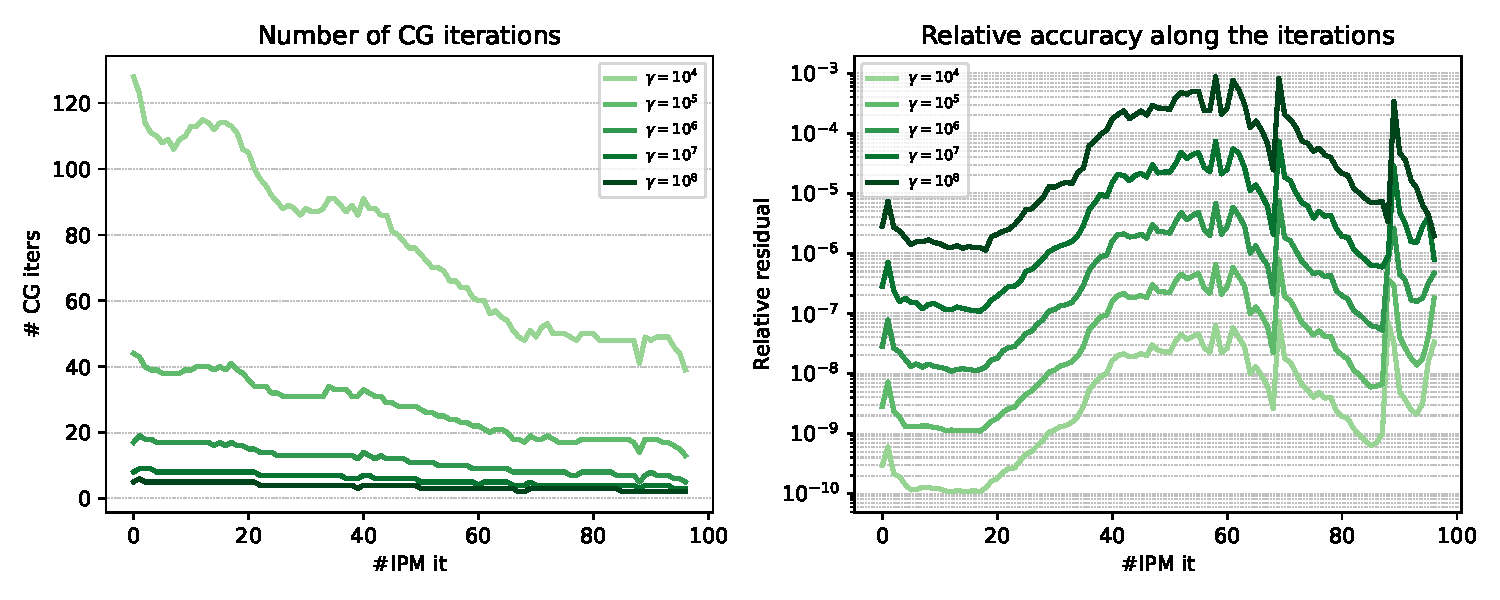
\includegraphics[width=\textwidth]{figures/hybrid-gamma.pdf}
  \caption{
    Above: Decomposition of IPM solution time across
    (a) condensation time (cond.), (b) \CG time, (c) total time
    spent in the linear solver (linsol.) and (d) total time spent in
    IPM solver (IPM).
    Below: Impact of $\gamma$ on the total number of \CG iterations
    and the norm of the relative residual at each IPM iteration.
    The peak observed in the norm of the relative residual corresponds
    to the primal-dual regularization performed inside the IPM algorithm,
    applied when the matrix $K_\gamma$ is not positive definite.
    \label{fig:hybrid:gamma}
  }
\end{figure}


\subsubsection{Tuning the equality relaxation strategy}
We now analyze the numerical performance of LiftedKKT (\S\ref{sec:kkt:sckkt}).
The method solves the KKT system~\eqref{eq:liftedkkt} using a direct solver.
The parameter $\tau$ used in the equality relaxation~\eqref{eq:problemrelaxation}
is set equal to the IPM tolerance $\varepsilon_{tol}$ (in practice, it does not
make sense to set a parameter $\tau$ below IPM tolerance as the
inequality constraints are satisfied only up to a tolerance $\pm \varepsilon_{tol}$
in IPM).

We compare in Table~\ref{tab:sckkt:performance} the performance obtained by LiftedKKT
as we decrease the IPM tolerance $\varepsilon_{tol}$.
We display both the runtimes on the CPU (using CHOLMOD-\ldlt) and on the GPU (using {\tt cuDSS}-\ldlt).
The slacks associated with the relaxed equality constraints are converging to a value below $2 \tau$,
leading to highly ill-conditioned terms in the diagonal matrices $D_s$.
As a consequence, the conditioning of the matrix $K_\tau$ in \eqref{eq:liftedkkt} can increase
above $10^{18}$, leading to a nearly singular linear system.
We observe {\tt cuDSS}-\ldlt is more stable than CHOLMOD: the factorization
succeeds, and the loss of accuracy caused by the ill-conditioning is tamed by the multiple
Richardson iterations that reduces the relative accuracy in the residual down to an acceptable level.
As a result, {\tt cuDSS} can solve
the problem to optimality in $\approx 20s$, a time comparable with HyKKT (see Figure~\ref{fig:hybrid:gamma}).

\begin{table}[!ht]
  \centering
  \resizebox{.7\textwidth}{!}{
  % \begin{tabular}{|l|rr|rr|rr|r|}
  %   \hline
  %   & \multicolumn{2}{c|}{\bf CHOLMOD-\ldlt (CPU)} & \multicolumn{2}{c|}{\bf LDLFactorizations (CPU)} & \multicolumn{2}{c|}{\bf cuDSS-\ldlt (CUDA)}& \\
  %   \hline
  %   $\varepsilon_{tol}$ & \#it & time (s)& \#it & time (s) & \#it & time (s) & accuracy \\
  %   \hline
  %   $10^{-4}$& 115 & 268.2  &220& 358.8& 114 & 19.9& $1.2 \times 10^{-2}$\\
  %   $10^{-5}$ & 210 & 777.8 & 120&  683.1& 113 & 30.4&$1.2 \times 10^{-3}$ \\
  %   $10^{-6}$ & 102 & 337.5 & 109&  328.7& 109 & 25.0&$1.2 \times 10^{-4}$  \\
  %   $10^{-7}$ &108 & 352.9 & 108&  272.9& 104 & 20.1&$1.2 \times 10^{-5}$ \\
  %   $10^{-8}$ & - &  - &- &  - & 105 & 20.3&$1.2 \times 10^{-6}$  \\
  %   \hline
  % \end{tabular}
  \begin{tabular}{|l|rr|rr|r|}
    \hline
    & \multicolumn{2}{c|}{\bf CHOLMOD-\ldlt (CPU)} & \multicolumn{2}{c|}{\bf cuDSS-\ldlt (CUDA)}& \\
    \hline
    $\varepsilon_{tol}$ & \#it & time (s)&  \#it & time (s) & accuracy \\
    \hline
    $10^{-4}$ & 115 & 268.2 & 114 & 19.9 & $1.2 \times 10^{-2}$ \\
    $10^{-5}$ & 210 & 777.8 & 113 & 30.4 & $1.2 \times 10^{-3}$ \\
    $10^{-6}$ & 102 & 337.5 & 109 & 25.0 & $1.2 \times 10^{-4}$ \\
    $10^{-7}$ & 108 & 352.9 & 104 & 20.1 & $1.2 \times 10^{-5}$ \\
    $10^{-8}$ & -   & -     & 105 & 20.3 & $1.2 \times 10^{-6}$ \\
    \hline
  \end{tabular}
  }
  \label{tab:sckkt:performance}
  \caption{Performance of the equality-relaxation
    strategy as we decrease the IPM tolerance $\varepsilon_{tol}$.
    The table displays the wall time on the CPU (using CHOLMOD-\ldlt)
    and on the GPU (using cuDSS-\ldlt).
  }
\end{table}

\subsubsection{Breakdown of the time spent in one IPM iteration}
We decompose the time spent in a single
IPM iteration for LiftedKKT and HyKKT.
As a reference running on the CPU, we show the time spent in the solver HSL MA27.
We observe that HSL MA57 is slower
than HSL MA27, as the OPF instances are super-sparse.
Hence, the block elimination algorithm implemented in HSL MA57 is not beneficial there
\footnote{Personal communication with Iain Duff.}.

When solving the KKT system, the time can be decomposed into: (1) assembling the
KKT system, (2) factorizing the KKT system, and (3) computing the descent direction with triangular solves.
As depicted in Figure~\ref{fig:timebreakdown}, we observe
that constructing the KKT system represents only a fraction of the computation time, compared
to the factorization and the triangular solves. Using {\tt cuDSS}-\ldlt, we observe speedups of
30x and 15x in the factorization compared to MA27 and CHOLMOD running on the CPU.
Once the KKT system is factorized, computing the descent direction with LiftedKKT is faster than with HyKKT
(0.04s compared to 0.13s) as HyKKT has to run a \CG algorithm to solve the Schur complement
system~\eqref{eq:kkt:schurcomplhykkt}, leading to additional backsolves
in the linear solver.

\begin{figure}[!ht]
  \centering
  \resizebox{.8\textwidth}{!}{
    \begin{tabular}{|l|rrrr|}
      \hline
       & build (s) & factorize (s) & backsolve (s) & accuracy \\
       \hline
      HSL MA27       & $3.15\times 10^{-2}$&$1.22 \times 10^{-0} $&$3.58\times 10^{-1}$&$5.52\times 10^{-7}$\\
      LiftedKKT (CPU)  & $8.71\times 10^{-2}$&$6.08\times 10^{-1}$&$2.32\times 10^{-1}$&$3.73\times 10^{-9}$\\
      HyKKT (CPU)  & $7.97\times 10^{-2}$&$6.02\times 10^{-1}$&$7.30\times 10^{-1}$&$3.38\times 10^{-3}$\\
      LiftedKKT (CUDA) & $2.09\times 10^{-3}$&$4.37\times 10^{-2}$&$3.53\times 10^{-2}$&$4.86\times 10^{-9}$\\
      HyKKT (CUDA) & $1.86\times 10^{-3}$&$3.38\times 10^{-2}$&$1.35\times 10^{-1}$&$3.91\times 10^{-3}$\\
      \hline
    \end{tabular}
  }
  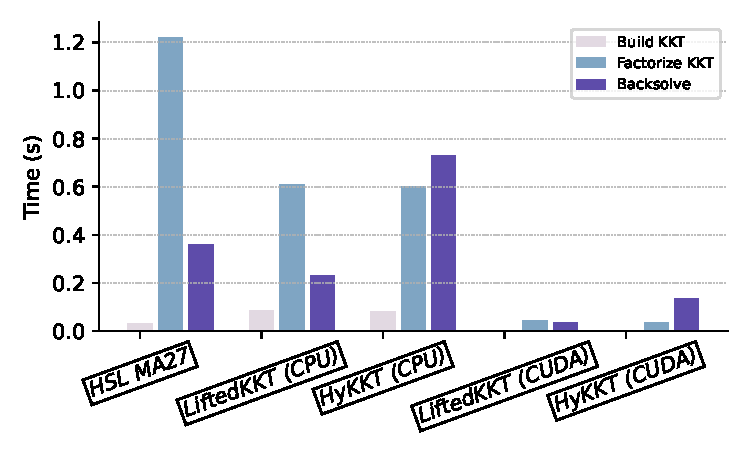
\includegraphics[width=.7\textwidth]{figures/breakdown.pdf}
  \caption{Breakdown of the time spent in one IPM iteration
    for different linear solvers, when solving {\tt 78484epigrids} (A30 GPU)
  \label{fig:timebreakdown}}
\end{figure}



\subsection{Benchmark on OPF instances}
\label{sec:num:opf}
We run a benchmark on difficult OPF instances taken
from the PGLIB benchmark~\cite{babaeinejadsarookolaee2019power}.
We compare LiftedKKT and HyKKT with HSL MA27.
The results are displayed in Table~\ref{tab:opf:benchmark},
for an IPM tolerance set to $10^{-6}$.
Regarding HyKKT, we set $\gamma = 10^7$ following the analysis in \S\ref{sec:num:tuninghykkt}.
The table displays the time spent in the initialization, the time spent in the linear solver and the total
solving time.
We complement the table with a Dolan \& Moré performance profile~\cite{dolan2002benchmarking} displayed
in Figure~\ref{fig:opf:pprof}.
Overall, the performance of HSL MA27 on the CPU is consistent with what was reported
in \cite{babaeinejadsarookolaee2019power}.

On the GPU, LiftedKKT+cuDSS is faster than HyKKT+cuDSS on small and medium instances: indeed, the algorithm
does not have to run a \CG algorithm at each IPM iteration, limiting the number
of triangular solves performed at each iteration.
Both LiftedKKT+cuDSS and HyKKT+cuDSS are significantly faster than HSL MA27.
HyKKT+cuDSS is slower when solving {\tt 8387\_pegase}, as on this particular instance
the parameter $\gamma$ is not set high enough to reduce the
total number of \CG iterations, leading to a 4x slowdown compared to LiftedKKT+cuDSS.
Nevertheless, the performance of HyKKT+cuDSS is better on the largest instances,
with almost an 8x speed-up compared to the reference HSL MA27.

The benchmark presented in Table~\ref{tab:opf:benchmark} has been generated using a
NVIDIA A100 GPUs (current selling price: \$10k). We have also compared the performance
with cheaper GPUs: a NVIDIA A1000 (a laptop-based GPU, 4GB memory) and a NVIDIA A30
(24GB memory, price: \$5k).
As a comparison, the selling price of the AMD EPYC
7443 processor we used for the benchmark on the CPU is \$1.2k. The results are
displayed in Figure~\ref{fig:gpubench}. We observe that the performance of the A30
and the A100 are relatively similar. The cheaper A1000 GPU is already faster
than HSL MA27 running on the CPU, but is not able to solve the largest instance as it is running out of memory.

\begin{table}[!ht]
  \centering
  \resizebox{\textwidth}{!}{
    \begin{tabular}{|l|rrr >{\bfseries}r|rrr >{\bfseries}r|rrr >{\bfseries}r|}
      \hline
      & \multicolumn{4}{c|}{\bf HSL MA27} &
      \multicolumn{4}{c|}{\bf LiftedKKT+cuDSS} &
      \multicolumn{4}{c|}{\bf HyKKT+cuDSS} \\
      \hline
      Case & it & init & lin & total & it & init & lin & total & it & init & lin & total \\
      \hline
      89\_pegase & 32 & 0.00 & 0.02 & 0.03 & 29 & 0.03 & 0.12 & 0.24 & 32 & 0.03 & 0.07 & 0.22 \\
      179\_goc & 45 & 0.00 & 0.03 & 0.05 & 39 & 0.03 & 0.19 & 0.35 & 45 & 0.03 & 0.07 & 0.25 \\
      500\_goc & 39 & 0.01 & 0.10 & 0.14 & 39 & 0.05 & 0.09 & 0.26 & 39 & 0.05 & 0.07 & 0.27 \\
      793\_goc & 35 & 0.01 & 0.12 & 0.18 & 57 & 0.06 & 0.27 & 0.52 & 35 & 0.05 & 0.10 & 0.30 \\
      1354\_pegase & 49 & 0.02 & 0.35 & 0.52 & 96 & 0.12 & 0.69 & 1.22 & 49 & 0.12 & 0.17 & 0.50 \\
      \hline
      2000\_goc & 42 & 0.03 & 0.66 & 0.93 & 46 & 0.15 & 0.30 & 0.66 & 42 & 0.16 & 0.14 & 0.50 \\
      2312\_goc & 43 & 0.02 & 0.59 & 0.82 & 45 & 0.14 & 0.32 & 0.68 & 43 & 0.14 & 0.21 & 0.56 \\
      2742\_goc & 125 & 0.04 & 3.76 & 7.31 & 157 & 0.20 & 1.93 & 15.49 & - & - & - & - \\
      2869\_pegase & 55 & 0.04 & 1.09 & 1.52 & 57 & 0.20 & 0.30 & 0.80 & 55 & 0.21 & 0.26 & 0.73 \\
      3022\_goc & 55 & 0.03 & 0.98 & 1.39 & 48 & 0.18 & 0.23 & 0.66 & 55 & 0.18 & 0.23 & 0.68 \\
      \hline
      3970\_goc & 48 & 0.05 & 1.95 & 2.53 & 47 & 0.26 & 0.37 & 0.87 & 48 & 0.27 & 0.24 & 0.80 \\
      4020\_goc & 59 & 0.06 & 3.90 & 4.60 & 123 & 0.28 & 1.75 & 3.15 & 59 & 0.29 & 0.41 & 1.08 \\
      4601\_goc & 71 & 0.09 & 3.09 & 4.16 & 67 & 0.27 & 0.51 & 1.17 & 71 & 0.28 & 0.39 & 1.12 \\
      4619\_goc & 49 & 0.07 & 3.21 & 3.91 & 49 & 0.34 & 0.59 & 1.25 & 49 & 0.33 & 0.31 & 0.95 \\
      4837\_goc & 59 & 0.08 & 2.49 & 3.33 & 59 & 0.29 & 0.58 & 1.31 & 59 & 0.29 & 0.35 & 0.98 \\
      \hline
      4917\_goc & 63 & 0.07 & 1.97 & 2.72 & 55 & 0.26 & 0.55 & 1.18 & 63 & 0.26 & 0.34 & 0.94 \\
      5658\_epigrids & 51 & 0.31 & 2.80 & 3.86 & 58 & 0.35 & 0.66 & 1.51 & 51 & 0.35 & 0.35 & 1.03 \\
      7336\_epigrids & 50 & 0.13 & 3.60 & 4.91 & 56 & 0.45 & 0.95 & 1.89 & 50 & 0.43 & 0.35 & 1.13 \\
      8387\_pegase & 74 & 0.14 & 5.31 & 7.62 & 82 & 0.59 & 0.79 & 2.30 & 75 & 0.58 & 7.66 & 8.84 \\
      9241\_pegase & 74 & 0.15 & 6.11 & 8.60 & 101 & 0.63 & 0.88 & 2.76 & 71 & 0.63 & 0.99 & 2.24 \\
      \hline
      9591\_goc & 67 & 0.20 & 11.14 & 13.37 & 98 & 0.63 & 2.67 & 4.58 & 67 & 0.62 & 0.74 & 1.96 \\
      10000\_goc & 82 & 0.15 & 6.00 & 8.16 & 64 & 0.49 & 0.81 & 1.83 & 82 & 0.49 & 0.75 & 1.82 \\
      10192\_epigrids & 54 & 0.41 & 7.79 & 10.08 & 57 & 0.67 & 1.14 & 2.40 & 54 & 0.67 & 0.66 & 1.81 \\
      10480\_goc & 71 & 0.24 & 12.04 & 14.74 & 67 & 0.75 & 0.99 & 2.72 & 71 & 0.74 & 1.09 & 2.50 \\
      13659\_pegase & 63 & 0.45 & 7.21 & 10.14 & 75 & 0.83 & 1.05 & 2.96 & 62 & 0.84 & 0.93 & 2.47 \\
      \hline
      19402\_goc & 69 & 0.63 & 31.71 & 36.92 & 73 & 1.42 & 2.28 & 5.38 & 69 & 1.44 & 1.93 & 4.31 \\
      20758\_epigrids & 51 & 0.63 & 14.27 & 18.21 & 53 & 1.34 & 1.05 & 3.57 & 51 & 1.35 & 1.55 & 3.51 \\
      30000\_goc & 183 & 0.65 & 63.02 & 75.95 & - & - & - & - & 225 & 1.22 & 5.59 & 10.27 \\
      78484\_epigrids & 102 & 2.57 & 179.29 & 207.79 & 101 & 5.94 & 5.62 & 18.03 & 104 & 6.29 & 9.01 & 18.90 \\
      \hline
    \end{tabular}
  }
  \caption{OPF benchmark, solved with a tolerance {\tt tol=1e-6}. (A100 GPU) \label{tab:opf:benchmark}}
\end{table}

\begin{figure}[!ht]
  \centering
  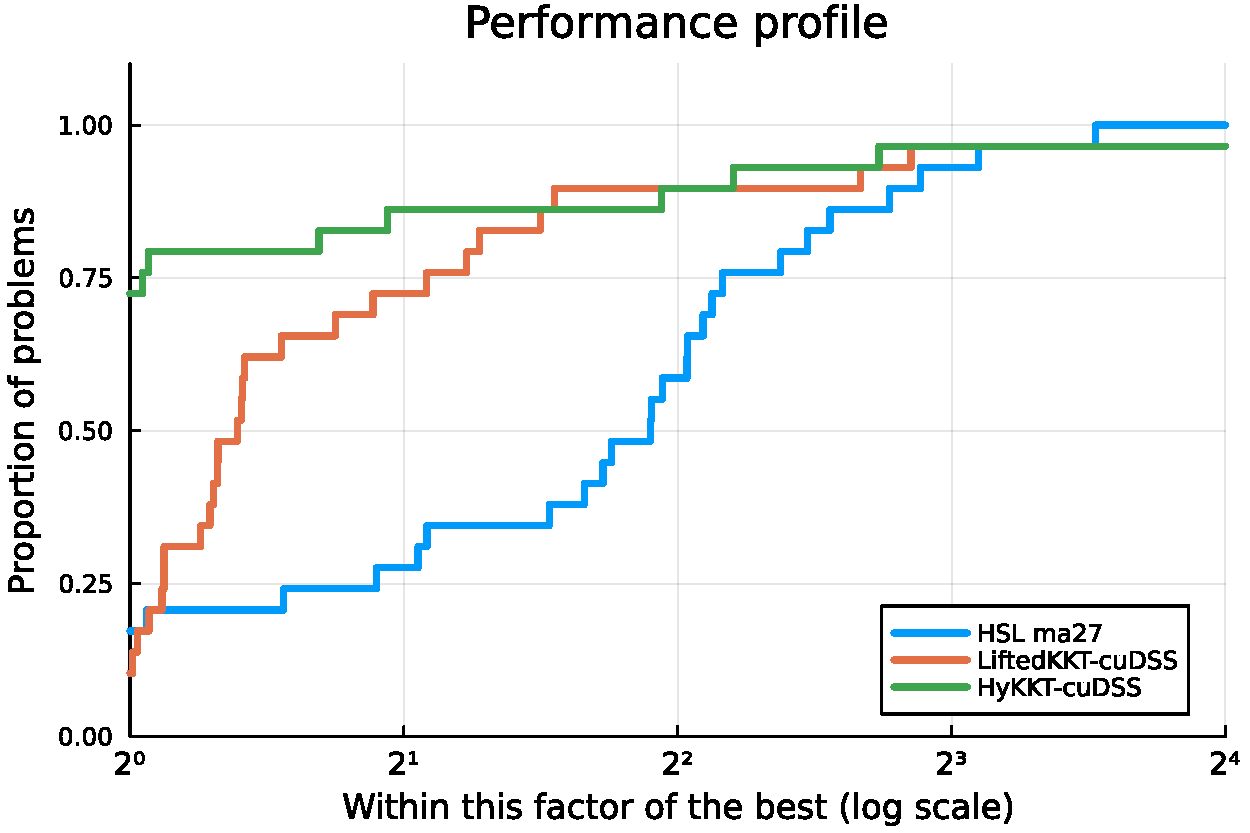
\includegraphics[width=.6\textwidth]{figures/pprof-cuda.pdf}
  \caption{Performance profile for the PGLIB OPF benchmark, solved
    with a tolerance {\tt tol=1e-6}.
  \label{fig:opf:pprof}}
\end{figure}

\begin{figure}[!ht]
  \centering
  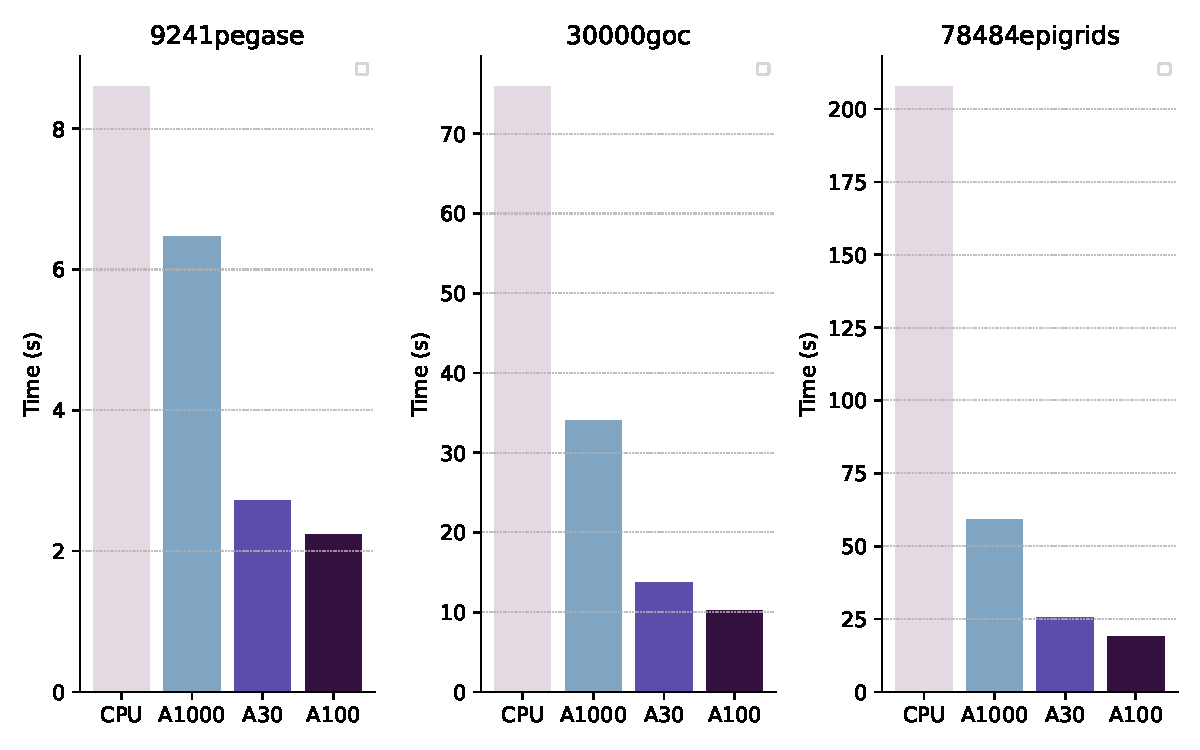
\includegraphics[width=.6\textwidth]{figures/benchmark_gpus.pdf}
  \caption{Comparing the performance obtained with various GPUs
    on three different OPF instances. We have used HyKKT to generate
    the results.
  \label{fig:gpubench}}
\end{figure}


\subsection{Benchmark on COPS instances}
\label{sec:num:cops}
We have observed in the previous section that both LiftedKKT
and HyKKT outperform HSL MA27 when running on the GPU.
However, the OPF instances are specific nonlinear instances.
For that reason, we complement our analysis by looking
at the performance of LiftedKKT and HyKKT on large-scale COPS instances~\cite{dolan2004benchmarking}.
We look at the performance we get on the COPS instances used in
the Mittelmann benchmark~\cite{mittelmann2002benchmark}.
To illustrate the heterogeneity of the COPS instances,
we display in Figure~\ref{fig:cops:nnz} the sparsity pattern of the
condensed matrices $K_\gamma$ \eqref{eq:kkt:hykkt} for one OPF instance and for multiple
COPS instances. We observe that some instances ({\tt bearing}) have a sparsity pattern
similar to the OPF instance on the left, whereas some are fully dense ({\tt elec}).
On the opposite, the optimal control instances ({\tt marine}, {\tt steering}) are
highly sparse and can be reordered efficiently using AMD ordering~\cite{amestoy-david-duff-2004}.

The results of the COPS benchmark are displayed in Table~\ref{tab:cops:benchmark}.
HSL MA57 gives better results than HSL MA27 for the COPS benchmark, and
for that reason we have decided to replace HSL MA27 by HSL MA57. As expected,
the results are different than on the OPF benchmark.
We observe that LiftedKKT+cuDSS and HyKKT+cuDSS outperform HSL MA57 on the dense instance {\tt elec}
(20x speed-up) and {\tt bearing}  --- an instance whose sparsity pattern
is similar to the OPF. In the other instances, LiftedKKT+cuDSS and HyKKT+cuDSS
on par with HSL MA57 and sometimes even slightly slower ({\tt rocket} and {\tt pinene}).


\begin{figure}[!ht]
  \centering
  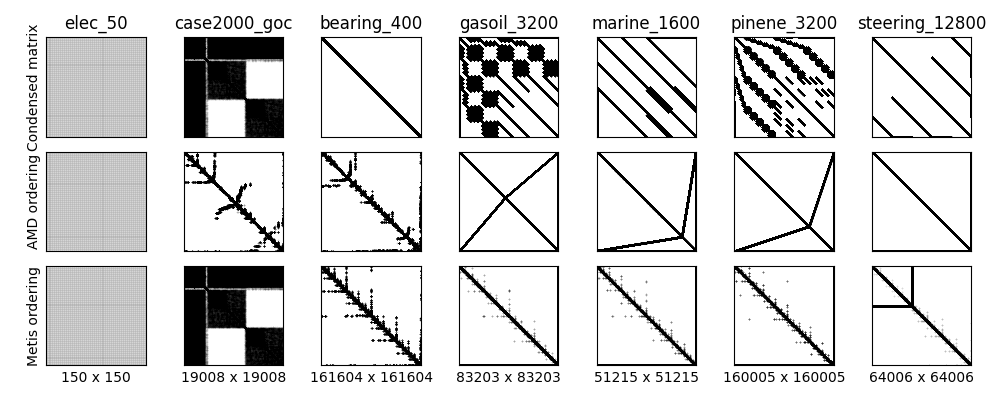
\includegraphics[width=.9\textwidth]{figures/sparsity_pattern.png}
  \caption{Sparsity patterns for one OPF instance and for various
    COPS problems. The first row displays the sparsity pattern
    of $K_\gamma$, after AMD reordering. The second row displays
    the sparsity pattern of $K_\gamma$ after Metis reordering.
    \label{fig:cops:nnz}
  }
\end{figure}


\begin{table}[!ht]
  \centering
  \resizebox{\textwidth}{!}{
    \begin{tabular}{|l|rr|rrr >{\bfseries}r|rrr >{\bfseries}r|rrr >{\bfseries}r|}
      \hline
  & &
  & \multicolumn{4}{c|}{\bf HSL MA57} &
      \multicolumn{4}{c|}{\bf LiftedKKT+cuDSS} &
      \multicolumn{4}{c|}{\bf HyKKT+cuDSS} \\
      \hline
      & $n$ & $m$ & it & init & lin & total & it & init & lin & total & it & init & lin & total \\
      \hline
      bearing\_400 & 162k & 2k & 17 & 0.14 & 3.42 & 4.10 & 14 & 0.85 & 0.07 & 1.13 & 14 & 0.78 & 0.76 & 1.74 \\
      camshape\_6400 & 6k & 19k & 38 & 0.02 & 0.18 & 0.29 & 35 & 0.05 & 0.03 & 0.19 & 38 & 0.05 & 0.04 & 0.23 \\
      elec\_400 & 1k & 0.4k & 185 & 0.54 & 24.64 & 33.02 & 273 & 0.46 & 0.97 & 20.01 & 128 & 0.48 & 0.75 & 4.16 \\
      gasoil\_3200 & 83k & 83k & 37 & 0.36 & 4.81 & 5.81 & 21 & 0.54 & 0.24 & 1.40 & 20 & 0.59 & 0.21 & 1.35 \\
      marine\_1600 & 51k & 51k & 13 & 0.05 & 0.41 & 0.50 & 33 & 0.38 & 0.58 & 1.29 & 13 & 0.37 & 0.12 & 0.62 \\
      pinene\_3200 & 160k & 160k & 12 & 0.11 & 1.32 & 1.60 & 21 & 0.87 & 0.16 & 1.52 & 11 & 0.90 & 0.84 & 2.02 \\
      robot\_1600 & 14k & 10k & 34 & 0.04 & 0.33 & 0.45 & 35 & 0.20 & 0.07 & 0.76 & 34 & 0.21 & 0.08 & 0.80 \\
      rocket\_12800 & 51k & 38k & 23 & 0.12 & 1.73 & 2.16 & 37 & 0.74 & 0.06 & 2.49 & 24 & 0.25 & 1.70 & 3.12 \\
      steering\_12800 & 64k & 51k & 19 & 0.25 & 1.49 & 1.93 & 18 & 0.44 & 0.06 & 1.64 & 18 & 0.46 & 0.07 & 1.83 \\
      \hline
      bearing\_800 & 643k & 3k & 13 & 0.94 & 14.59 & 16.86 & 14 & 3.31 & 0.18 & 4.10 & 12 & 3.32 & 1.98 & 5.86 \\
      camshape\_12800 & 13k & 38k & 34 & 0.02 & 0.34 & 0.54 & 33 & 0.05 & 0.02 & 0.16 & 34 & 0.06 & 0.03 & 0.19 \\
      elec\_800 & 2k & 0.8k & 354 & 2.36 & 337.41 & 409.57 & 298 & 2.11 & 2.58 & 24.38 & 184 & 1.81 & 2.40 & 16.33 \\
      gasoil\_12800 & 333k & 333k & 20 & 1.78 & 11.15 & 13.65 & 18 & 2.11 & 0.98 & 5.50 & 22 & 2.99 & 1.21 & 6.47 \\
      marine\_12800 & 410k & 410k & 11 & 0.36 & 3.51 & 4.46 & 146 & 2.80 & 25.04 & 39.24 & 11 & 2.89 & 0.63 & 4.03 \\
      pinene\_12800 & 640k & 640k & 10 & 0.48 & 7.15 & 8.45 & 21 & 4.50 & 0.99 & 7.44 & 11 & 4.65 & 3.54 & 9.25 \\
      robot\_12800 & 115k & 77k & 35 & 0.54 & 4.63 & 5.91 & 33 & 1.13 & 0.30 & 4.29 & 35 & 1.15 & 0.27 & 4.58 \\
      rocket\_51200 & 205k & 154k & 31 & 1.21 & 6.24 & 9.51 & 37 & 0.83 & 0.17 & 8.49 & 30 & 0.87 & 2.67 & 10.11 \\
      steering\_51200 & 256k & 205k & 27 & 1.40 & 9.74 & 13.00 & 15 & 1.82 & 0.19 & 5.41 & 28 & 1.88 & 0.56 & 11.31 \\
      \hline
    \end{tabular}
  }
  \caption{COPS benchmark , solved with a tolerance {\tt tol=1e-6}\label{tab:cops:benchmark}}
\end{table}


%%% Local Variables:
%%% mode: latex
%%% TeX-master: "../main"
%%% End:



\section{Conclusion}
Future extensions:
\begin{itemize}
  \item Interplay with first-order method (PDHG for LP)
  \item Solving LP and QP problems on the GPU with IPM
  \item From Cholesky to LDL (regularization can
    ensure the KKT matrix is SQD, c.f. Orban, Saunders).
\end{itemize}

\bibliographystyle{siam}
\bibliography{biblio.bib}

\end{document}
